\documentclass[aspectratio=169,10pt]{beamer}
\usetheme{Madrid}
\usecolortheme{default}

\usepackage[utf8]{inputenc}
\usepackage[T1]{fontenc}
\usepackage{amsmath,amssymb}
\usepackage{booktabs}
\usepackage{graphicx}
\usepackage{tikz}
\usetikzlibrary{patterns,shapes,arrows.meta,calc,positioning}
\usepackage{listings}
\usepackage{hyperref}

% --- Skema Warna Khas UNIB / Optimisasi ---
\definecolor{unibblue}{RGB}{0,51,102}
\definecolor{unibgold}{RGB}{212,175,55}
\definecolor{unibgreen}{RGB}{0,128,0}
\definecolor{codebg}{RGB}{244,247,251}

\setbeamercolor{structure}{fg=unibblue}
\setbeamercolor{palette primary}{bg=unibblue,fg=white}
\setbeamercolor{palette secondary}{bg=unibblue!85,fg=white}
\setbeamercolor{palette tertiary}{bg=unibblue!70,fg=white}
\setbeamercolor{block title}{bg=unibblue!90,fg=white}
\setbeamercolor{block body}{bg=unibblue!8,fg=black}
\setbeamercolor{alertblock title}{bg=unibgold!90,fg=black}
\setbeamercolor{alertblock body}{bg=unibgold!14,fg=black}
\setbeamercolor{exampleblock title}{bg=unibgreen!85,fg=white}
\setbeamercolor{exampleblock body}{bg=unibgreen!8,fg=black}

\lstset{
  language=Python,
  basicstyle=\ttfamily\scriptsize,
  backgroundcolor=\color{codebg},
  frame=single,
  rulecolor=\color{unibblue!35},
  keywordstyle=\color{unibblue}\bfseries,
  commentstyle=\color{unibgreen!80!black}\itshape,
  stringstyle=\color{red!60!black},
  showstringspaces=false,
  breaklines=true
}

\title[Aliran Daya Python — Modul 1]{Analisis Aliran Daya Menggunakan Python}
\subtitle{Modul 1: Pemodelan Jaringan \& Pembentukan Matriks Admitansi Bus ($Y_{\text{bus}}$)}
\author[Novalio Daratha]{Novalio Daratha\\Program Studi Teknik Elektro, Universitas Bengkulu}
\date{Workshop Teknis Intensif (32 JP) — 2026}

\begin{document}

\begin{frame}
  \titlepage
\end{frame}

\begin{frame}{Agenda Modul 1 (8 JP)}
  \tableofcontents
\end{frame}

\section{Tujuan Pembelajaran \& Peta Kurikulum}

\begin{frame}{Tujuan Pembelajaran Modul 1 (Taksonomi Bloom C1--C5)}
  \begin{block}{Capaian Pembelajaran Modul}
    \begin{itemize}
      \item \textbf{[C1]} Mengklasifikasikan tiga tipe bus (\textit{Slack}, \textit{PV}, \textit{PQ}) beserta besaran diketahui dan dicari.
      \item \textbf{[C2]} Menjelaskan model saluran nominal-$\pi$ dan transformator \textit{off-nominal tap / phase-shifter}.
      \item \textbf{[C3]} Menerapkan normalisasi sistem per-unit dan membangun fungsi \texttt{build\_ybus()} sparse.
      \item \textbf{[C4]} Menganalisis sifat sparsitas, simetri, dan dampak \textit{phase-shifter} terhadap $Y_{\text{bus}}$.
      \item \textbf{[C5]} Memvalidasi silang hasil $Y_{\text{bus}}$ terhadap pustaka referensi industri (\texttt{pandapower}).
    \end{itemize}
  \end{block}
  \vspace{0.2cm}
  \begin{center}
    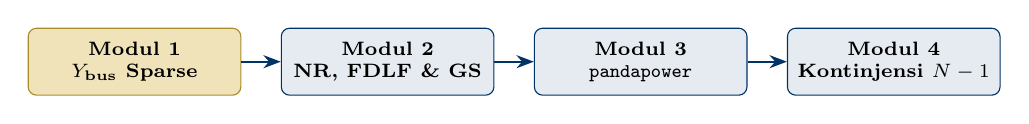
\begin{tikzpicture}[
      box/.style={draw=unibblue, fill=unibblue!10, rounded corners=3pt, minimum width=2.7cm, minimum height=0.85cm, align=center, font=\scriptsize\bfseries},
      arr/.style={-{Stealth[length=2.2mm]}, thick, color=unibblue}
    ]
      \node[box, fill=unibgold!35, draw=unibgold!80!black] (m1) {Modul 1\\$Y_{\text{bus}}$ Sparse};
      \node[box, right=0.5cm of m1] (m2) {Modul 2\\NR, FDLF \& GS};
      \node[box, right=0.5cm of m2] (m3) {Modul 3\\\texttt{pandapower}};
      \node[box, right=0.5cm of m3] (m4) {Modul 4\\Kontinjensi $N-1$};
      \draw[arr] (m1) -- (m2);
      \draw[arr] (m2) -- (m3);
      \draw[arr] (m3) -- (m4);
    \end{tikzpicture}
  \end{center}
\end{frame}

\section{Sistem Per-Unit \& Klasifikasi Bus}

\begin{frame}{Normalisasi Per-Unit \& Tipe Bus Aliran Daya}
  \begin{columns}[T]
    \begin{column}{0.46\textwidth}
      \begin{block}{Sistem Per-Unit ($S_{\text{base}} = 100\text{ MVA}$)}
        \[
          Z_{\text{base}} = \frac{V_{\text{base,LL}}^{2}}{S_{\text{base}}},\qquad
          z_{\text{pu}} = \frac{Z_{\Omega}}{Z_{\text{base}}}
        \]
        \[
          z_{\text{pu}}^{\text{baru}} = z_{\text{pu}}^{\text{lama}}\left(\frac{V_{\text{base}}^{\text{lama}}}{V_{\text{base}}^{\text{baru}}}\right)^{2}\frac{S_{\text{base}}^{\text{baru}}}{S_{\text{base}}^{\text{lama}}}
        \]
      \end{block}
      \begin{exampleblock}{Keunggulan Komputasi}
        Trafo dengan rasio nominal menghilang dari model; yang tersisa hanya deviasi tap (\textit{off-nominal tap}).
      \end{exampleblock}
    \end{column}
    \begin{column}{0.52\textwidth}
      \textbf{Klasifikasi 3 Jenis Bus Utama:}
      \vspace{0.15cm}
      \scriptsize
      \begin{tabular}{@{}llll@{}}
        \toprule
        \textbf{Tipe Bus} & \textbf{Diketahui} & \textbf{Dicari} & \textbf{Peran Fisik} \\
        \midrule
        \textbf{Slack (REF)} & $|V|,\,\theta=0$ & $P,\,Q$ & Penutup rugi \& referensi sudut \\
        \textbf{PV (Gen)} & $P,\,|V|$ & $Q,\,\theta$ & Generator dgn AVR ($Q_{\min}\!\le\!Q\!\le\!Q_{\max}$) \\
        \textbf{PQ (Beban)} & $P,\,Q$ & $|V|,\,\theta$ & Beban konstan / PV terkunci batas $Q$ \\
        \bottomrule
      \end{tabular}
      \vspace{0.25cm}
      \normalsize
      \begin{alertblock}{Injeksi Daya Bersih Terjadwal}
        $S_i^{\text{sch}} = (P_{G,i} - P_{D,i}) + j(Q_{G,i} - Q_{D,i})$
      \end{alertblock}
    \end{column}
  \end{columns}
\end{frame}

\section{Model Cabang Nominal-$\pi$ \& Trafo Bertap}

\begin{frame}{Model Umum Cabang: Saluran Nominal-$\pi$ + Trafo Kompleks}
  \begin{center}
    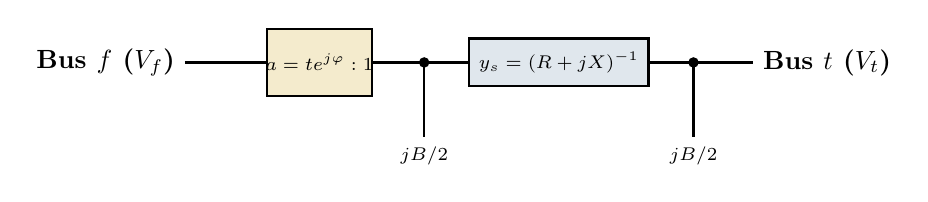
\begin{tikzpicture}[scale=0.95, transform shape]
      \draw[thick] (0,0) node[left] {\textbf{Bus $f$ ($V_f$)}} -- (1.1,0);
      \draw[thick, fill=unibgold!25] (1.1,-0.45) rectangle (2.5,0.45);
      \node at (1.8,0) {\scriptsize $a = t e^{j\varphi} : 1$};
      \draw[thick] (2.5,0) -- (3.8,0);
      \draw[thick, fill=unibblue!12] (3.8,-0.32) rectangle (6.2,0.32);
      \node at (5.0,0) {\scriptsize $y_s = (R + jX)^{-1}$};
      \draw[thick] (6.2,0) -- (7.6,0) node[right] {\textbf{Bus $t$ ($V_t$)}};
      \draw[thick] (3.2,0) -- (3.2,-1.0) node[below] {\scriptsize $jB/2$};
      \draw[thick] (6.8,0) -- (6.8,-1.0) node[below] {\scriptsize $jB/2$};
      \fill (3.2,0) circle (2pt); \fill (6.8,0) circle (2pt);
    \end{tikzpicture}
  \end{center}
  \begin{block}{Matriks Admitansi Dua-Kutub Cabang ke-$l$}
    \[
      \begin{bmatrix} I_f \\ I_t \end{bmatrix} =
      \begin{bmatrix}
        \dfrac{y_s + j\frac{B}{2}}{|a|^2} & -\dfrac{y_s}{a^*} \\[8pt]
        -\dfrac{y_s}{a} & y_s + j\frac{B}{2}
      \end{bmatrix}
      \begin{bmatrix} V_f \\ V_t \end{bmatrix}
      =
      \begin{bmatrix} Y_{ff} & Y_{ft} \\ Y_{tf} & Y_{tt} \end{bmatrix}
      \begin{bmatrix} V_f \\ V_t \end{bmatrix}
    \]
  \end{block}
  \begin{alertblock}{Dampak \textit{Phase-Shifter} ($\varphi \neq 0$)}
    Karena $a \neq a^*$, maka $Y_{ft} \neq Y_{tf}$ sehingga matriks $Y_{\text{bus}}$ menjadi \textbf{tidak simetris}!
  \end{alertblock}
\end{frame}

\section{Perakitan Matriks Sparse dengan SciPy}

\begin{frame}[fragile]{Formulasi Insidensi \& Implementasi \texttt{scipy.sparse.csr\_matrix}}
  \begin{columns}[T]
    \begin{column}{0.44\textwidth}
      \begin{block}{Persamaan Insidensi Tervektorisasi}
        \begin{align*}
          Y_f &= \operatorname{diag}(Y_{ff}) C_f + \operatorname{diag}(Y_{ft}) C_t \\
          Y_t &= \operatorname{diag}(Y_{tf}) C_f + \operatorname{diag}(Y_{tt}) C_t \\
          Y_{\text{bus}} &= C_f^{\mathsf{T}} Y_f + C_t^{\mathsf{T}} Y_t + \operatorname{diag}(Y_{\text{sh}})
        \end{align*}
      \end{block}
      \begin{exampleblock}{Mengapa Wajib \textit{Sparse}?}
        Pada 10.000 bus, $>99{,}95\%$ entri bernilai nol. Memori turun dari $O(N^2)$ ke $O(N+L)$.
      \end{exampleblock}
    \end{column}
    \begin{column}{0.54\textwidth}
      \textbf{Cuplikan Inti \texttt{ybus.py}:}
\begin{lstlisting}
a = tap * np.exp(1j * np.deg2rad(shift))
y_tt = y_s + 0.5j * b_c
y_ff = y_tt / (np.abs(a) ** 2)
y_ft = -y_s / np.conj(a)
y_tf = -y_s / a

rows = np.concatenate([f, f, t, t, idx_b])
cols = np.concatenate([f, t, f, t, idx_b])
vals = np.concatenate([y_ff, y_ft, y_tf, y_tt, y_sh])
y_bus = sp.coo_matrix((vals, (rows, cols)),
                      shape=(n_bus, n_bus)).tocsr()
\end{lstlisting}
    \end{column}
  \end{columns}
\end{frame}

\section{Tugas Lab, Titik Periksa \& Rubrik}

\begin{frame}{Rencana Lab Hands-On 1 \& Titik Periksa IEEE 14-Bus}
  \begin{columns}[T]
    \begin{column}{0.54\textwidth}
      \begin{block}{Aktivitas Praktikum (3,5 Jam)}
        \begin{enumerate}
          \item \textbf{Lab 1.1 (C3):} Hitung $Y_{\text{bus}}$ sistem 3-bus secara manual.
          \item \textbf{Lab 1.2 (C3):} Bangun \texttt{make\_ybus()} sparse tervektorisasi (dukung nomor bus acak \texttt{bus\_map}).
          \item \textbf{Lab 1.3 (C4):} Plot pola sparsitas (\texttt{plt.spy}) dan uji efek \textit{phase-shifter} $5^\circ$ pada T4--7.
          \item \textbf{Lab 1.4 (C5):} Validasi silang terhadap \texttt{pandapower} dengan galat $<10^{-10}$.
        \end{enumerate}
      \end{block}
    \end{column}
    \begin{column}{0.44\textwidth}
      \begin{exampleblock}{Titik Periksa IEEE 14-Bus}
        \begin{itemize}
          \item Dimensi: $14 \times 14$
          \item Elemen tak-nol (\texttt{nnz}): \textbf{54} (densitas $27{,}55\%$)
          \item $Y_{11} = 6{,}0250 - j19{,}4471\text{ p.u.}$
          \item Simetri ($\varphi=0$): \texttt{True} ($\|Y-Y^{\mathsf{T}}\|_\infty = 0$)
        \end{itemize}
      \end{exampleblock}
      \begin{alertblock}{Bobot Rubrik Modul 1 (15\%)}
        Hitung manual (15\%), Kebenaran fungsi (35\%), Efisiensi sparse (20\%), Analisis sifat (20\%), Validasi (10\%).
      \end{alertblock}
    \end{column}
  \end{columns}
\end{frame}

\begin{frame}{Terima Kasih — Lanjut ke Modul 2}
  \begin{center}
    \vspace{0.8cm}
    {\Large \textbf{Terima Kasih}}\\
    \vspace{0.4cm}
    {\large Sesi Tanya Jawab \& Praktikum \texttt{python3 ybus.py}}\\
    \vspace{1.2cm}
    Novalio Daratha\\
    Program Studi Teknik Elektro, Universitas Bengkulu\\
    \texttt{https://ndaratha.my.id/w-pf/}
  \end{center}
\end{frame}

\end{document}
